
\chapter{Standard Model and neutrino phenomenology}\label{cap:introduccion}

\section{Standard Model}

The standard model is the theory that relates elementary particles and fundamental forces. This model explains how these elementary particles build matter and how they are affected by force fields.
\\
\begin{figure}[h!]
    \centering
    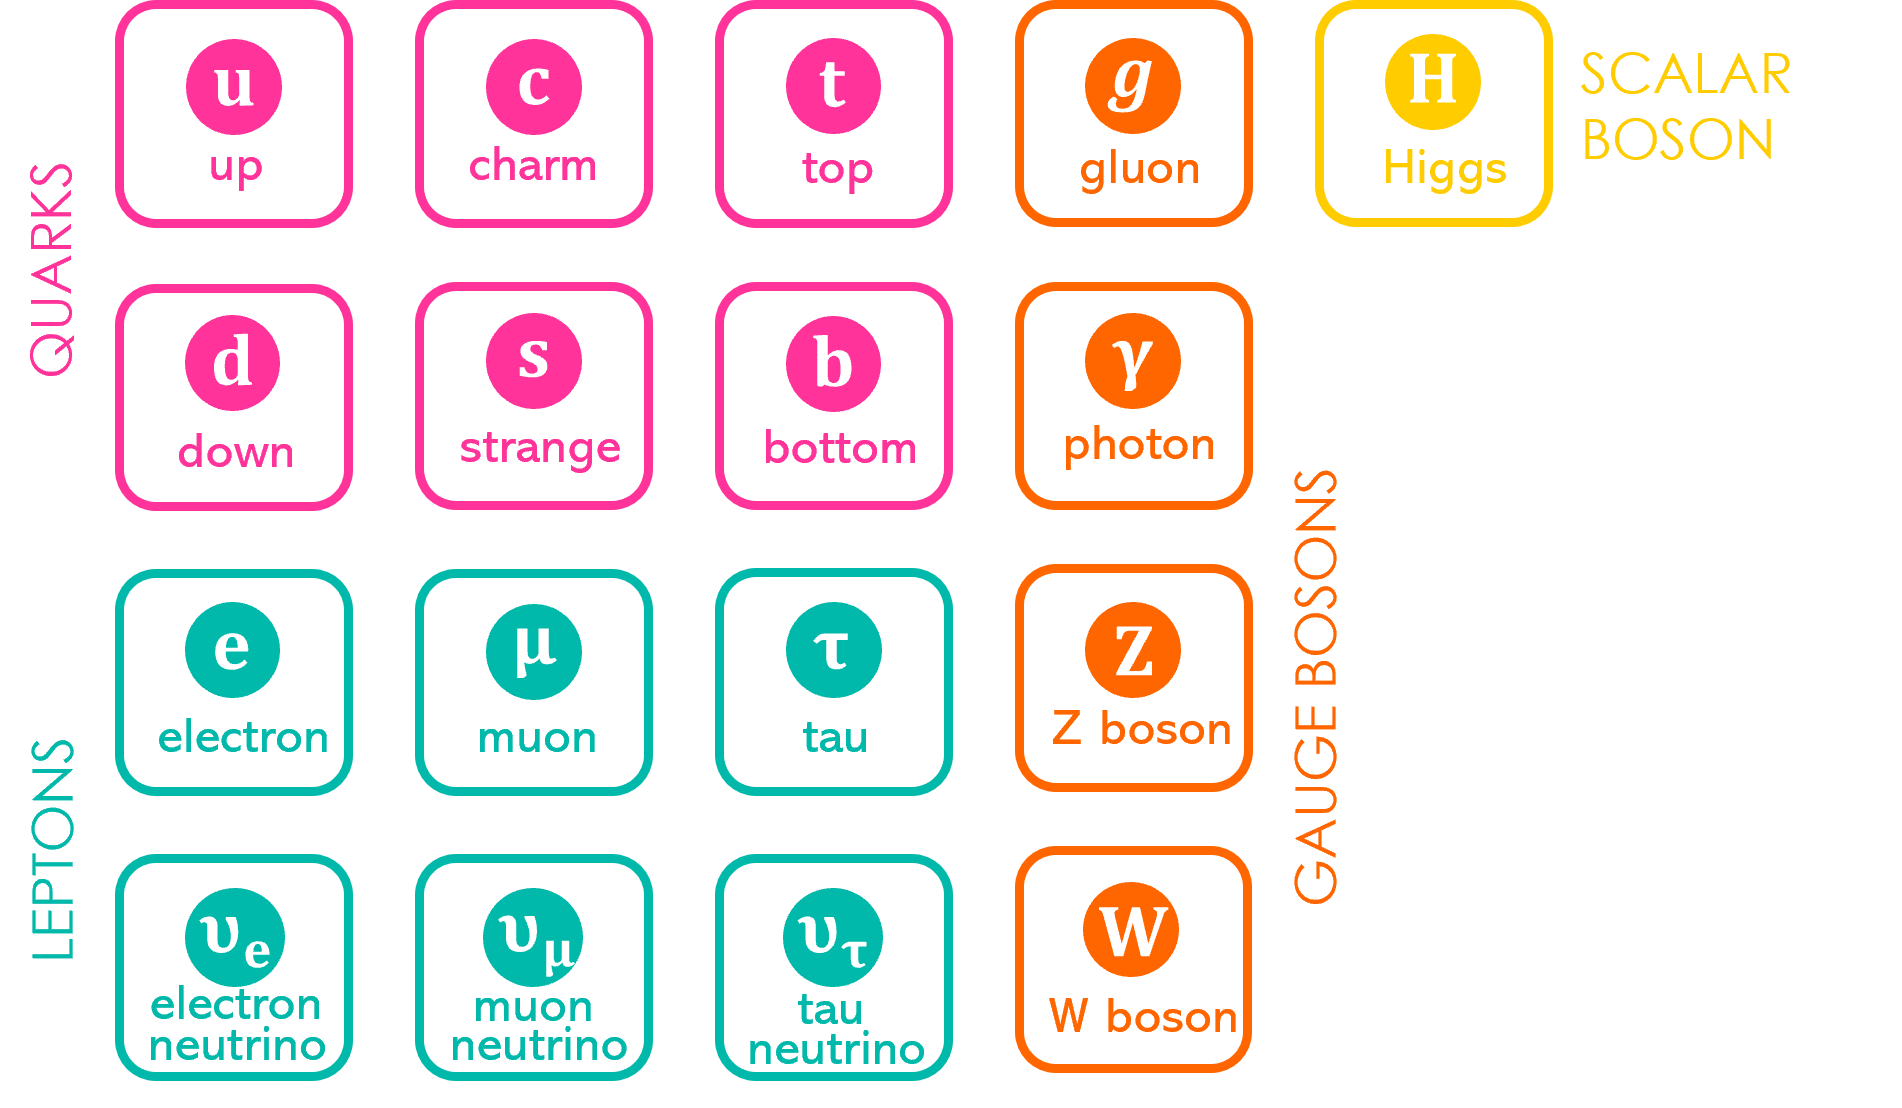
\includegraphics[scale=0.9]{figures/Imagen2.png}
    \caption{Elementary particles of the Standard Model}
    \label{fig1}
\end{figure}
\\
We call them elementary particles because, until now, they have not been considered composed of sub-particles. Some particles,  such as leptons and quarks, constitute matter, while others are responsible for carrying and mediating the fundamental forces that affect matter particles. These force-carrying particles are known as gauge bosons and include the photon (mediating the electromagnetic force), the gluon (mediating the strong interaction), and the W/Z bosons (mediating weak interactions). Additionally, we have the Higgs boson, which is a scalar boson. There are six quarks flavors. Five of them are components of composite particles known as hadrons. Furthermore, we have three families of leptons, which are the electron (e), the muon ($\mu$), and the tau ($\tau$), each with its respective neutrino ($\nu_e, \nu_\mu, \nu_\tau$). These particles and some of their properties can be observed in figure \ref{fig1}.

These last particles are the ones of our interest, as they only interact weakly, making them very difficult to be detected (despite being very abundant in the universe) since the probability of these interactions occurring is very low. In fact, the effective cross-section of these interactions is very small, on the order of $1\times10^{-44} cm^2$, compared to that of other processes.

\section{Neutrino interactions}
Neutrinos are tiny particles that were long believed to be massless. However, the discovery of neutrino oscillations revealed otherwise, although the precise value of their masses remains uncertain. Nevertheless, it is established that neutrinos are exceptionally lightweight particles, significantly lighter than the next lightest particle, the electron. Furthermore, it is established that the three distinct types of neutrinos possess different masses.

Despite their abundance in the universe, neutrinos present a formidable challenge when it comes to their detection due to their minimal interaction with matter. Neutrinos primarily engage through the weak nuclear force, resulting in exceedingly small cross-sections for their interactions, typically on the order of $10^{-44} cm^2$. In comparison, interactions like those involving the electromagnetic force can have cross-sections on the order of $10^{-25} cm^2$. The significant difference in interaction strength demands specialized detectors and techniques to capture neutrinos' elusive interactions.
\newpage
\begin{figure}[h!]
    \centering
    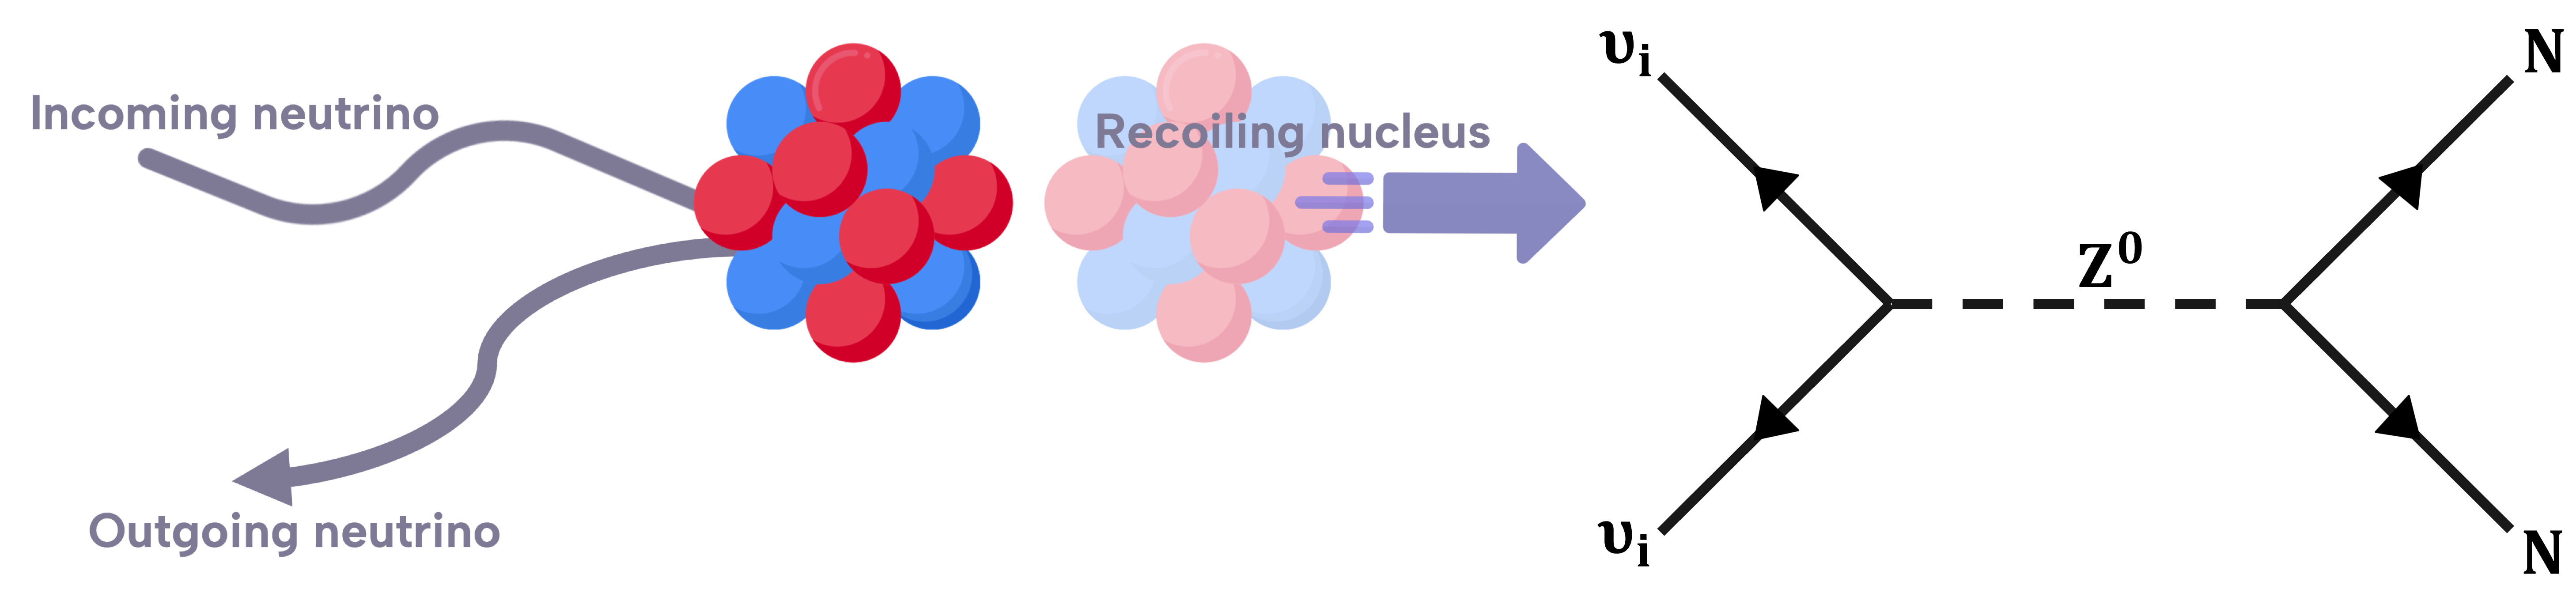
\includegraphics[scale=0.076]{figures/image.png}
    \caption{Coherent elastic neutrino-nucleus scattering \cite{science.aao4050}}
    \label{fig2}
\end{figure}

Neutrino interactions can be classified as charged current (CC) interactions, where neutrinos exchange a $W^{+/-}$ boson, and neutral current (NC) interactions, where a $Z$ boson is exchanged.

We are interested in the interactions of neutrinos with nuclei, which can also be classified by the energy range in which they occur. At high energies of around $\sim TeV$, deep inelastic scattering occurs, where the neutrino scatters off a quark, resulting in a high transfer of momentum inside the nucleon and causing the interaction to destroy the nucleon, making it an inelastic interaction \cite{doi:10.1146/annurev-nucl-102115-044720}. Conversely, nuclear excitation takes place at intermediate energies.\\
On the other hand, at low energies of around $\sim KeV$, coherent elastic neutrino-nucleus scattering (CE$\nu$NS) occurs, where the neutrino collides with a nucleus, and since it carries such low energy, the nucleus only experiences a small recoil as a whole (Figure \ref{fig2}). This process is coherent even up to an energy of 50 MeV (for an average-sized nucleus), as the condition for coherence is that the momentum transfer is small, that is, less than the inverse of the nucleus radius \cite{Scholberg_2020}.



The coherent nature of this process results in a relatively large cross-section compared to other neutrino interaction processes, as illustrated in Figure \ref{fig3},  where different total cross-sections for different neutrino interaction processes are compared. However, the challenge in detecting it lies in the fact that the recoil of the nuclei involved is minimal, typically on the order of a few KeV. The detection then requires the use of highly sensitive detectors. Consequently, despite CE$\nu$NS being proposed as early as 1974 \cite{Freedman}, its first observation occurred relatively recently, achieved by the COHERENT collaboration in 2017 \cite{Akimov_2017}.

\begin{figure}[h!]
    \centering
    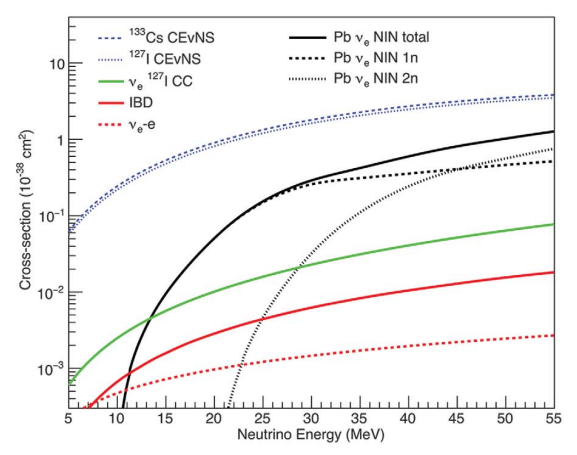
\includegraphics[scale=1]{figures/Captura.PNG}
    \caption{Total cross-sections from CE$\nu$NS and other neutrino interactions \cite{Akimov_2017}.}
    \label{fig3}
\end{figure}

\section{Neutrino oscillations}

The energy source for the Sun and stars is attributed to the fusion process, in which lighter elements merge to create heavier elements. For the Sun, this fusion involves the conversion of hydrogen into helium. To be more precise, within the solar interior, four hydrogen nuclei, known as protons $(p)$, undergo a transformation, resulting in the formation of a helium nucleus $(^4He)$, two positrons $(e^+)$, and two neutrinos $(\nu_e)$ \cite{Roxburgh}.
This fusion reaction follows a specific form.
\begin{equation*}
    ^4p \rightarrow  {^4{He}} + 2e^+ + 2\nu_e.
\end{equation*}
Due to their weak interactions, it was initially assumed that these low-energy neutrinos could pass through the Sun and reach the Earth without undergoing any alterations. Therefore, measuring the energy spectrum of neutrinos was believed to provide valuable information about the conditions in which nuclear reactions occur within the Sun.

In 1968, Raymond Davis Jr. and his team conducted the detection of solar neutrinos at the Homestake Mine in South Dakota \cite{Cleveland_1998}. Their approach involved using a substantial 600-ton tank filled with a chlorine-rich compound strategically located at a depth of 1350 meters to reduce interference from cosmic radiation. The detection of these neutrinos involved the inverse reaction of beta decay:
\begin{equation*}
    \nu_e + {^{37}_{17}Cl} \rightarrow e^- + {^{37}_{18}Ar^*}.
\end{equation*}
The notation $Ar^*$ indicates that the produced argon is radioactive, facilitating its detection through radiochemical methods; this allows for the estimation of the number of neutrinos that have interacted in the tank over a certain period.
Because of the low interaction rate, data collection for this experiment spanned multiple years, with an occurrence of roughly one neutrino interaction in the tank every two days. To everyone's surprise, the number of detected neutrinos was approximately one-third of the expected value. This disparity between the measured and calculated neutrino flux is recognized as the "solar neutrino deficit" or the solar neutrino problem.

Three potential explanations for this phenomenon were proposed. The first possible explanation is that the theoretical calculations were incorrect, which could occur if either the predicted number of neutrinos or the calculated production rate of argon atoms were inaccurate. The second possibility is that there were errors in the experiment. The third and most audacious possibility is that physicists did not fully comprehend the neutrinos' behavior when they travel astronomical distances.

In 1989, the Kamiokande experiment, led by Masatoshi Koshiba and Yoji Totsuka, aimed to address the solar neutrino problem \cite{BUGAEV1989391}. They used a large water detector to measure high-energy neutrinos emitted by the Sun. The experiment confirmed that the observed number of neutrino events was lower than predicted, but the discrepancy was less severe than in previous experiments.
In the following decade, three more experiments further revealed the mystery. GALLEX \cite{ANSELMANN1992376} and SAGE \cite{ABDURASHITOV1994234}, led by Till Kirsten and Vladimir Gavrin, respectively, utilized gallium detectors to show that lower-energy neutrinos were also missing. This was significant because it allowed for more accurate calculations of low-energy neutrinos.
Additionally, the Super-Kamiokande experiment, led by Totsuka and Yochiro Suzuki, made more precise measurements of high-energy neutrinos and confirmed the initial deficit observed \cite{Super.81.1158}. Therefore, it became clear that both high- and low-energy neutrinos were missing, although in different proportions.

Overall, these experiments highlighted the persistent discrepancy between the observed and predicted number of neutrino events, adding complexity to the solar neutrino problem.

In June 2001, a collaboration of Canadian, American, and British scientists led by Arthur McDonald announced the resolution of the solar neutrino mystery. They used the Solar Neutrino Observatory (SNO), a 1,000-ton heavy water detector in Sudbury, Ontario, to obtain the first solar neutrino results \cite{SNO}.


In order to explain the change in neutrino flavors during propagation, it is crucial to consider that flavor eigenstates $\ket{\nu_\alpha}$, in general, are not mass eigenstates of the mass operator M. This means that $\braket{\nu_\alpha|M|\nu_\beta}\neq0$ for $\alpha\neq\beta$. Instead, flavor eigenstates are composed of combinations of non-degenerate mass eigenstates $\ket{\nu_i}$ with $\braket{\nu_i|M|\nu_j}=m_i\delta_{ij}$  and $m_i-m_j\neq 0$ for $i\neq j$ . Neutrino oscillations can occur because the mixing amplitude A is non-zero for flavor B.

Flavor and mass eigenstates are related through a unitary transformation U known as the mixing matrix, similar to the CKM matrix. In the Standard Model, where all neutrinos are considered massless, the matrix U has no physical significance. Hence, by incorporating the mixing matrix, we implicitly assume that at least one of the neutrinos does not have a mass different from zero.

Thus, these eigenstates could be represented as linear combinations in the following form:
\begin{equation}
    \ket{\nu_\alpha} = \sum_i U^*_{\alpha i} \ket{\nu_i}
\end{equation}
and
\begin{equation}
    \ket{\nu_i} = \sum_\alpha U_{\alpha i} \ket{\nu_\alpha},
    \label{masstates}
\end{equation}

here the two basis are orthonormal $\braket{\nu_i|\nu_j}=\delta_{ij}$ and $\braket{\nu_\alpha|\nu_\beta}=\delta_{\alpha \beta}$. Using the unitary relation $U^\dagger U=1$
\begin{equation}
\sum_\alpha U^*_{\alpha i} U_{\alpha j} =\delta_{ij}.
\end{equation}
Since there are three active flavor neutrinos $(\nu_e,\nu_\mu,\nu_\tau)$, the minimum number of massive neutrinos is also three. If there are more than three massive neutrinos, the additional neutrinos in the flavor basis are considered sterile \cite{10.1093/acprof:oso/9780198508717.001.0001}.

The massive neutrino states are eigenstates of the Hamiltonian operator:
\begin{equation}
    \mathcal{H}\ket{\nu_i}=E_i\ket{\nu_i}.
\end{equation}
With energy eigenvalues $E_i=\sqrt{p^2+m_i^2}$  .The mass states of neutrinos evolve in time according to 
\begin{equation}
    \ket{\nu_i (t)} =e^{-iE_i t}\ket{\nu_i}.
\end{equation}
Therefore, a flavor state that describes a neutrino created with a definite flavor $\alpha$ at time t=0 will evolve with time into the state :
\begin{equation}
    \ket{\nu_\alpha(t)}=\sum_k{U^*_{\alpha i}e^{-iE_it}\ket{\nu_i}}.
\end{equation}
By substituting equation \ref{masstates}
\begin{equation*}
    \ket{\nu_\alpha(t)}=\sum_\beta \left( \sum_i U^*_{\alpha i}e^{-iE_i t}U_{\beta i} \right) \ket{\nu_\beta}.
\end{equation*}
This equation demonstrates that the neutrino state at a time t, initially created with a defined flavor $\alpha$, evolves into a superposition of the different neutrino flavor states at $t>0$. The coefficient of $\ket{\nu_\beta}$ is the transition amplitude as a function of time
\begin{equation*}
    A_{\nu_\alpha \rightarrow \nu_\beta} (t) \equiv \braket{\nu_\beta|\nu_\alpha(t)} =\sum_i U^*_{\alpha i} U_{\beta i} e^{iE_i t},
\end{equation*}
then, the probability of finding the neutrino on a  flavor state $\ket{\nu_\beta}$ is given by
\begin{equation}
    P_{\nu_\alpha\rightarrow\nu_\beta}(t)=|A_{\nu_\alpha \rightarrow \nu_\beta} (t)|^2 =\sum_{i,j} U^*_{\alpha i} U_{\beta i} U_{\alpha j} U^*_{\beta j} e^{-i(E_i -E_j) t}.
\end{equation}
Given that the detected neutrinos have very small masses, they have been considered ultra-relativistic. Moreover, is possible to  make the following approximation:
\begin{align}
    E_i&\approx E +\frac{m_i^2}{2E}, & E_i-E_j\approx& \frac{\Delta m^2_{ij}}{2E},
\end{align}
$\Delta m^2_{ij}\equiv m_i^2-m_j^2$ stands for the squared-mass difference. E is the neutrino energy for a neglectable mass contribution.  Thus, the transition probability can be approximated by
\begin{equation*}
    P_{\nu_\alpha\rightarrow\nu_\beta}(t)=\sum_{i,j} U^*_{\alpha i} U_{\beta i} U_{\alpha j} U^*_{\beta j} e^{-i\frac{\Delta m^2_{ij}t}{2E}}.
\end{equation*}
The final step in deriving this oscillation probability is the conversion of time to distance. Since experiments do not measure the propagation time; we only know the distance L between the source and detector. This conversion can be achieved by using natural units, where $t\approx L$, resulting in
\begin{equation}
    P_{\nu_\alpha\rightarrow\nu_\beta}(L,E)=\sum_{i,j} U^*_{\alpha i} U_{\beta i} U_{\alpha j} U^*_{\beta j} e^{-i\frac{\Delta m^2_{ij}L}{2E}}.
\end{equation}
These expressions show that the oscillation probability is only sensitive to the squared mass difference of the neutrinos $(\Delta m^2_{ij})$.

